\documentclass[a4paper,10pt]{article}
\usepackage[left=2cm,right=2cm,top=3.0cm,bottom=3cm]{geometry}
\usepackage[brazilian]{babel}
\usepackage[utf8]{inputenc}
\usepackage[T1]{fontenc}
\usepackage{graphicx}
\usepackage{subfig}
\usepackage{amssymb}
\usepackage{amsmath}
\usepackage[colorlinks=true,linkcolor=black,linktoc=all, urlcolor=black]{hyperref}
\usepackage{fancyhdr}
\usepackage{amsmath,amssymb,exscale}	%inserir eq e simbolos matemáticos
\usepackage{bbm, dsfont}

%\usepackage{helvet}
\renewcommand{\familydefault}{\sfdefault}


\date{}
\title{
    O Uso de Redes de Petri na Modelagem de \\Workflows Científicos e seus Recursos\footnote{Este trabalho foi financiado por uma bolsa de iniciação científica RUSP (processo número: ?????).}
}

\author{
\textbf{\textit{Duílio Henrique Haroldo Elias}},\textbf{ \textit{Kelly Rosa Braghetto}}\\
\\
\textit{Universidade de São Paulo} / \textit{Instituto de Matemática e Estatística}\\
\\
\href{mailto:duilio.elias@usp.br}{duilio.elias@usp.br} | \href{mailto:kellyrb@ime.usp.br}{kellyrb@ime.usp.br}
}


% Define o rodapé e o cabeçalho
\fancyhf{} 
\renewcommand{\headrulewidth}{0pt}
\cfoot{SIICUSP 2014 -- 22º Simpósio Internacional de Iniciação Científica e Tecnológica da USP }
\pagestyle{fancy}

\begin{document}
\maketitle
    
\section*{Resumo}
%*** Na primeira página deve ficar apenas os resumos em português e em inglês. \\
%O texto deve ter um total de 4 páginas. ***
	Nas últimas décadas os workflows científicos receberam grande atenção da comunidade acadêmica, devido à sua grande
capacidade de manipulação, análise e simulação de experimentos que trabalham com grandes quantidades de dados. No entanto,
as ferramentas existentes para tal fim são ainda escassas e muitos cientistas afirmam que esse seja o é um grande gargalo da produção científica. Neste trabalho, busca-se contribuir com este processo, criando modelos estocásticos capazes de descrever analiticamente alguns workflows bem estudado pela comunidade acadêmica. Com isso, pretende-se extrair índices capazes de predizer o impacto do uso de diferentes abordagens de controle de fluxo de dados no desempenho dos workflows.

\section*{Abstract}

In the last decades, scientific workflows received great attention from the academic community, due to its large handling capability, analysis and simulation of experiments with large amounts of data. However, existing tools for this purpose are still scarce and many scientists claim that this is the major difficulty of the  scientific production. In this work, we try to contribute to this process by creating stochastic models capable of describing analytically some workflows well studied by the academic community. With this, we intend to extract indexes able to predict the impact of using different approaches to control data flow in the performance of workflows.

\thispagestyle{fancy}

\newpage

\section*{Introdução}
%O Que são workflow científicos? OK

Um workflow científico(WfC) pode ser compreendido como um conjunto de tarefas computacionais que constituem um experimento científico \cite{Junior2012}, ou seja, os passos a serem executados pelo experimento. Os WfCs são conhecidos pelo seu poder de manipulação e execução de experimentos científicos automatizáveis que trabalham com grandes quantidades de dados o que os caracterizam como uma estruturas baseadas no fluxo de dados, ou seja, baseadas nas conexões entre as atividades e as dependência entre elas. Conceitualmente, um WfC pode ser visto como um grafo dirigido onde os nós são aplicações componentes e as arestas representam os fluxos de dados. Esse grafo pode ser acíclico, indicando que o WfC não contem controle de fluxo do tipo laço, onde um mesmo trecho do WfC poderia ser repetido até que alguma condição fosse satisfeita. Por \textit{aplicações componentes}, entende-se como um programa de computador que implemente uma tarefa de um experimento científico computacional\cite{Junior2012}. Um experimento pode ser composto por diversos WfC, que seguem um ciclo de vida.\\

	%Por que eles são importantes?	
	As aplicações de WfCs são bastante extensas e a maioria delas visam automatizar processos computacionais complexos, assim como aumentar o desempenho dos mesmos.
	
	 %Que ferramentas de apoio possuem? OK 	%Como eles são modelados? ok
	As principais etapas do ciclo de vida de um WfC são a modelagem, execução e análise e são normalmente gerenciadas por sistemas complexos chamados de Sistemas Gerenciadores de Workflows Científicos(SGWfC). A especificação de um WfC pode ser através de uma \textit{linguagem de workflow} ou por meio de uma \textit{interface gráfica} que permita aos cientistas sem muito conhecimento avançados de computação especificar o workflow de forma mais fácil. Hoje existem diversos SGWfC e cada um deles apresentam particularidades para representação dos WfC que visam atender necessidades especificas de cada área. Os SGWfC mais utilizados, segundo o número compartilhamento no myexperiment\footnote{http://www.myexperiment.org/}, repositório de WfC, são:
	
	\begin{itemize}
	
		\item \textbf{Taverna}\footnote{http://www.taverna.org.uk/}: Tem como foco aparar cientistas da área de Ciências Biológicas é uma ferramenta multiplataforma e possue uma boa documentação. O Taverna possue uma interface gráfica que permite ao pesquisador construir WfC de forma muito parecida com fluxogramas e possuem suporte a \textit{Web Services}.

		\item \textbf{Pegasus}\footnote{http://pegasus.isi.edu/}: O Pegasus é uma que permite aparar diversas áreas, permite a construção de WfC em sistemas distribuídos, também é uma solução multiplataforma, porém não possue uma interface gráfica intuitiva como o Taverna e os WfC são descritos em formato XML, na linguagem DAX que descreve as dependências entre atividades e os recursos computacionais, onde cada aplicação componente será executada.

		\item \textbf{Kepler} \footnote{https://kepler-project.org/}: Assim como o Taverna o Kepler é uma ferramenta voltada para área de Bioinformática e os WfCs pode ser descritos com o auxílio de uma interface gráfica e também é uma ferramenta multiplataforma.

	\end{itemize}
	
	Estes são os principais SGWfC e estão descritos bem sucintamente, porém cada um tem suas particularidades que visam atender a necessidades especificas de cada área e cada cientista precisa escolher o que mais atende as suas necessidades. 

	%Porque é interessante modelar workflows usando linguagens formais como Redes de Petri (verificação de propriedades dos modelos, extração de índices de desempenho, etc.)
		Para este trabalho escolhemos o Pegasus, por ter uma boa documentação e permitir modelar sistemas com recursos computacionais distribuídos e também por possuir toda descrição em modo textual(DAX), que poderá no futuro criar um algoritmo para modelagem analítica de forma a automatizar criação de modelos analíticos que será feita nas próximas seções.

\section*{Objetivos}

O objetivo deste trabalho é definir um método de conversão de modelos de workflows baseados em fluxos de dados(WfC) em modelos em Rede de Petri Estocásticas. Para isso foram modelados um grupo de WfC, o qual se conhece bem o comportamento, utilizando para isso o arquivo DAX, neste arquivo é possível obter o tempo de execução de cada atividade, o tamanho de cada arquivo compartilhado e a precedência entre as atividades. Com essas informações foi possível construir as redes de Petri correspondentes. Em modelos em Rede de Petri Estocásticas, pode-se também incorporar informações sobre o taxa de execução das atividades e sobre os recursos computacionais disponíveis para a execução do WfC; por essa razão, é possível extrair deles predições sobre o desempenho do WfC.


\section*{Materiais e Métodos}
	
	As Redes Petri(RdP) são um dos formalismos mais utilizados para modelagem analítica e análise de sistemas concorrentes mais utilizados, e isso deve-se à fácil compreensão, representação gráfica e devido ao seu potencial matemático para análise de modelos. Algumas características importantes de WfC podem ser facilmente representadas utilizando RdP, tais como a sincronização de tarefas, concorrência e controle de dependências\cite{Braghetto2011}.
	Uma RdP pode ser formalmente definida pela tupla $RdP={L,T,A,P,m_{0}}$, em que:

		\begin{itemize}
		\item $L=\{l_{1},l_{2},...,l_{L}\}$ é um conjunto de lugares;
		\item $T=\{t_{1},t_{2},...,t_{T}\}$ é um conjunto de transições;
		\item $A\subseteq(L x T)\bigcup (TxL)$ é um conjunto de arcos;
		\item $P:A\rightarrow\mathbbm{N}$ é a função peso dos arcos;
		\item $m_{0}=\{m_{01},m_{02},...,m_{0L}\}$ é a marcação inicial da rede;
		\end{itemize}

	Cada uma dessas definições está associados a diferentes e importantes conceitos de RdP, que são:
		
		\begin{itemize}
			
			\item \textit{lugar} (representado graficamente por um círculo)- modela uma condição que deve ser satisfeita para que o disparo da transição seja realizado;

			\item \textit{transição} (representado graficamente por um retângulo) - pode ser compreendido por uma por uma ação ou um evento;

			\item \textit{arco orientado} liga um lugar a uma transição ou o contrário, ligando condições e eventos;

			\item \textit{fichas, marcas ou tokens} (representado por um ponto preto)- Representam um recurso ou um estado de um sistema;

			\item \textit{peso} - os arcos possuem um peso associado a eles; os pesos indica quantas fichas uma transição consome de um lugar de entrada ou quantas fichas uma transição acrescenta em um lugar de saída. Por \textit{default} quando um arco não possui um peso o peso é 1;
					
			\end{itemize}
			
Da necessidade de modelagem de sistemas grandes e complexos, como os encontrados na natureza e na sociedade, foram definidas sobre a base de Redes de Petri clássica outras redes de alto nível, como as Redes de Petri Temporizadas(RdPTs) e Redes de Petri Estocásticas(RdPEs). As RdPTs como o nome diz, permite modelar situações que ocorrem entre o início e fim de cada tarefa em termos do tempos. O que permitiu diferentes possibilidades para modelagem, como lugares temporizados, fichas temporizadas e todas as outras estruturas descritas acima puderam ser temporizadas e permitiram modelar uma série de sistemas reais. Já as RdPEs é uma subclasse das RdPTs, onde o tempo de atraso de uma transição é uma variável aleatória exponencialmente distribuída\cite{Braghetto2011}. \\
		
	Ao se usar as redes de Petri para se modelar a execução de um workflow, cada vértice pode armazenar um ou mais tokens, os vértices de transição de redes de Petri podem consumir e produzir tokens de múltiplas localizações. Os vértices de transições agem em tokens de entrada por um processo denominado disparo. Quando uma transição é disparada, ela consome os tokens de suas posições de entrada, realiza alguma tarefa de processamento, e realoca um número específico de tokens nas suas posições de saída. Isso é feito atomicamente. Como os disparos são não-determinísticos, as redes de Petri são muito utilizadas para modelar comportamento concorrente em sistemas distribuídos\cite{Ogasawara2011}, como é possível associar a cada transição uma taxa de disparo, ou seja, isto representará o inverso do tempo gasto para executar determinada atividade no WfC.\\
	
	Em uma RdPE, cada atividade do WfC é modelada como uma transição e cada transição do WfC é modelada como um lugar. Porém em algumas ocasiões precisa-se construir estruturas auxiliares como é o caso para \textit{\textbf{Paralelismo(4)}} criado na figura \ref{RdPE_Montage} para representar entradas de dados simultâneas.	\\


		As principais construções de fluxo de dados estão descritas abaixo e exemplificadas na figura \ref{RdPE_Montage} como é feita a modelagem analítica usando Redes de Petri Estocásticas(RdPE):
		
	\begin{itemize}
		
		\item \textit{Pipeline(1)}: são várias atividades combinadas sequencialmente, em que cada atividade recebe como entrada os dados produzidos como saída da atividade anterior;
		
		\item \textit{Agregação de dados(2)}: é feita por atividades que processam múltiplos conjuntos de dados de entrada, gerando uma combinação dos dados como saída;

		\item \textit{Distribuição de dados(3)}: é feita por atividades que produzem dados de saída que são recebidos como entrada por múltiplas atividades, ou que apenas particionam grandes conjuntos de dados em subconjuntos menores para serem processados por outras atividades no workflow;

	\end{itemize}

	\begin{figure}[!htb]
		\centering
		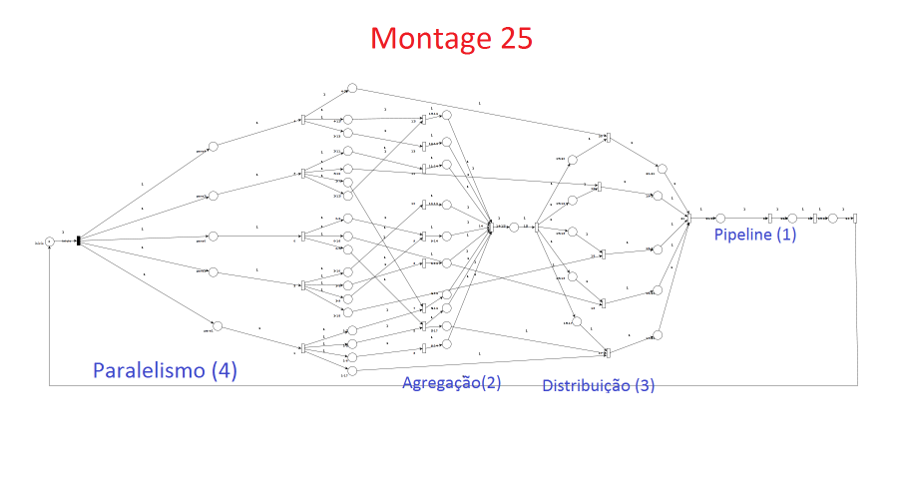
\includegraphics{img/montage25_peq}
		\caption{Exemplo de RdPE}
		\label{RdPE_Montage}
	\end{figure}

	Como estudo de caso, foi usado um conjunto de WfCs sintéticos (extraídos de workflows reais) que ilustram o uso de diferentes construções de fluxos de dados e que com frequência são empregados como base de comparação \footnote{https://confluence.pegasus.isi.edu/display/pegasus/WorkflowGenerator}. Estes WfCs estão descritos na linguagem DAX; seus modelos já trazem informações sobre o tempo médio de execução de cada atividade e também sobre o tamanho dos dados de entrada. Essas informações são importantes na construção das RdPEs e foram utilizados neste trabalho.\\
	
	Para representação dos recursos computacionais disponíveis em RdPT foi criado um lugar,uma transição de ida e uma volta para cada atividade da RdP e para representar de cada máquina foram colocados tokens, ou seja, para cada maquina um token. Poderia-se também para representar o tempo transferência de dados, colocar uma taxa de transição em cada uma das transições que liga uma atividade ao lugar das máquinas. Para modelagem e análise numérica das redes criadas foi utilizada o PIPE que é uma ferramenta \textit{Open Source} que permite criar modelos gráficos de RdPEs e possue módulos para análise numérica do modelo e extrair de imediato dois índices de desempenho interessantes: a porcentagem de utilização dos recursos e o rendimento(throughput) das atividades e do WfC.
	
\section*{Resultados}
	Para cada WfC sintético foi feita a sua modelagem em RdPE como o auxílio do PIPE e estão disponíveis \url{http://www.ime.usp.br/~kellyrb/ic/#duilio}, observe na figura \ref{Epigenomics_WfC} a representação gráfica do \textit{Epigenomics 24} \footnote{http://en.wikipedia.org/wiki/Epigenomics} que é um estudo sobre modificações reversíveis no DNA, que estão ligadas a diversos processos celulares e na figura \ref{Epigenomics_RdPE} a modelagem analítica usando RdPE.

\begin{figure}[!h]
	\centering
	\subfloat[WfC]{
		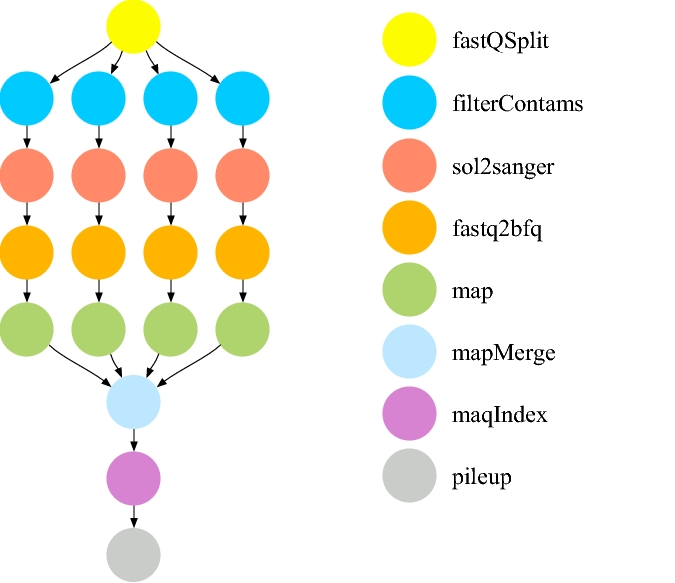
\includegraphics[height=5cm]{img/Epigenomics}
		\label{Epigenomics_WfC}
	}
	\quad %espaco separador
	\subfloat[RdPE]{
		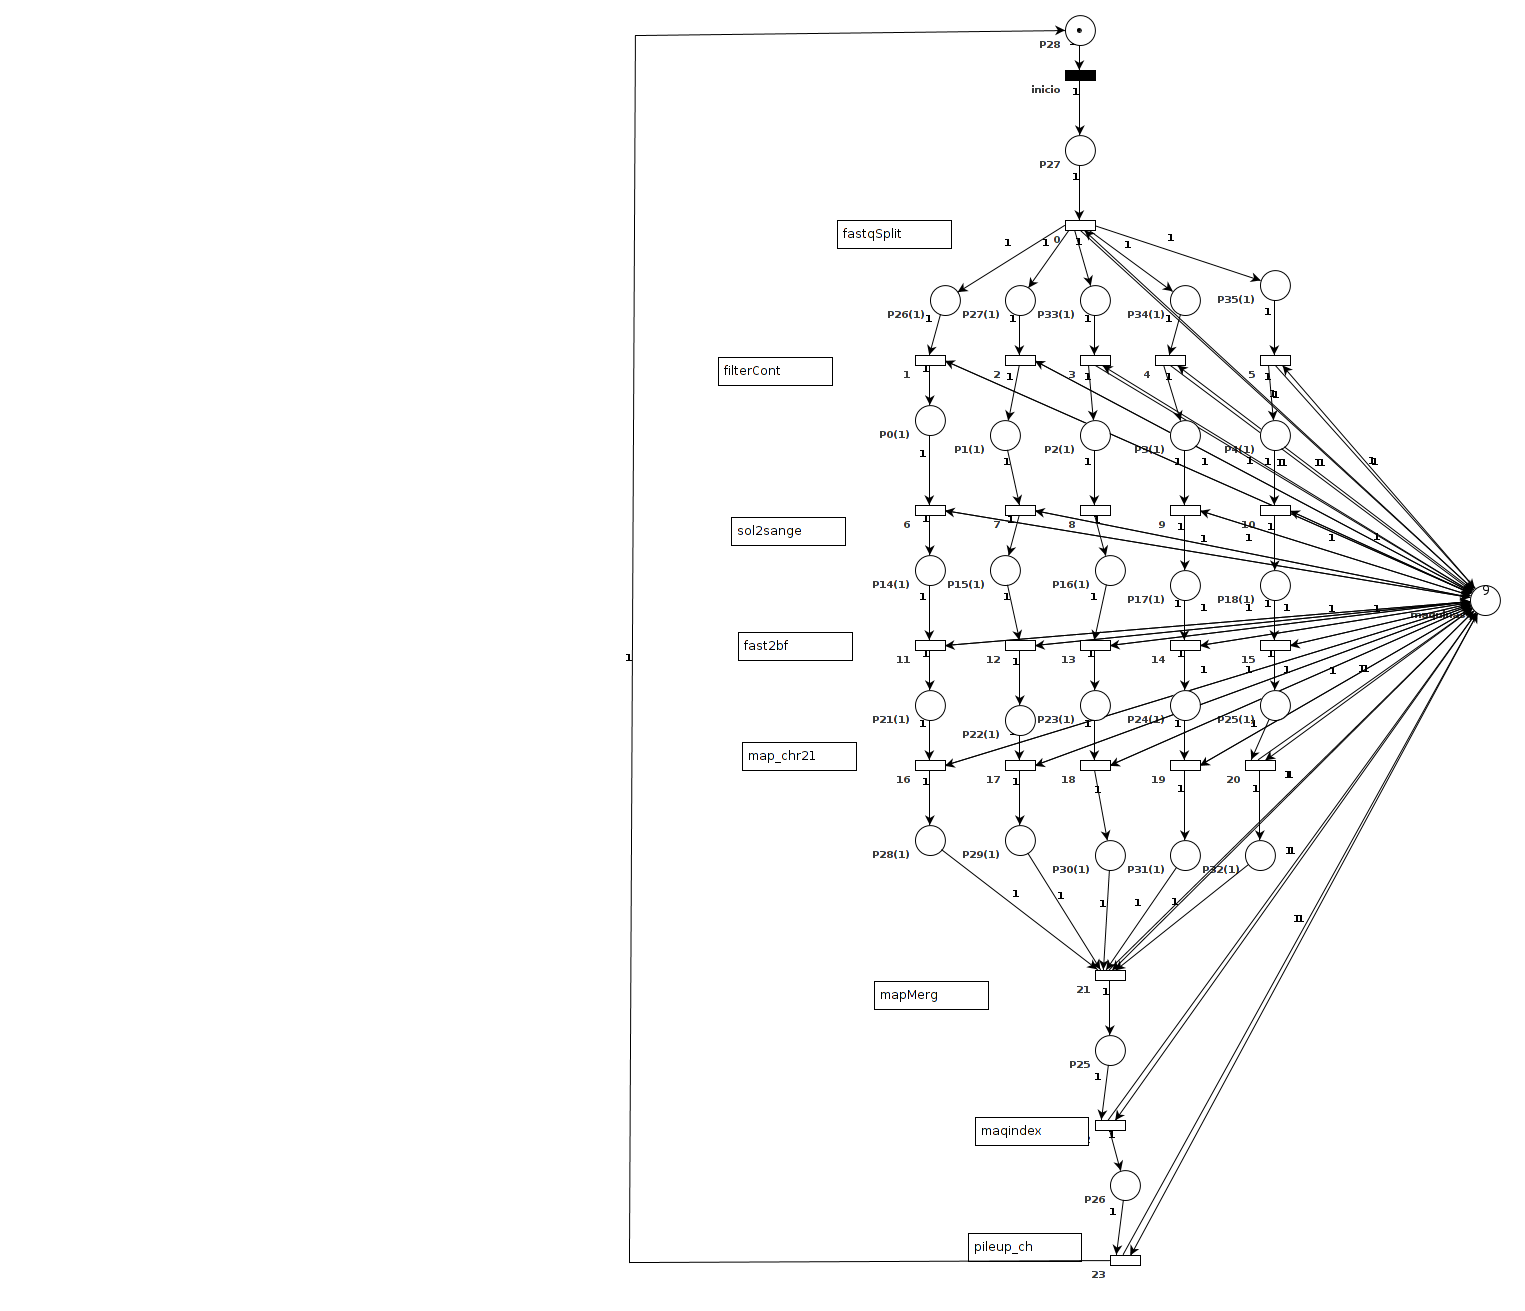
\includegraphics[height=5cm]{img/Epigenomics_RdPE}
		\label{Epigenomics_RdPE}
	}
	\caption{Modelagem Analítica do Epigenomics}
	\label{modelagem_analitica}
\end{figure}
\newpage

\section*{Conclusões}

Neste trabalho, foram modelados em RdP um conjunto de workflows científicos sintéticos (extraídos de workflows reais) que ilustram o uso de diferentes construções de fluxos de dados. Concluiu-se que, por meio das Redes de Petri, é possível representar todas as construções básicas de fluxos de dados, além de recursos computacionais simples (como máquinas, VMs, processadores) são facilmente expressos nos modelos em RdP. A solução numérica dos modelos em RdP traz uma predição do desempenho do workflow (utilização dos recursos e o rendimento (throughput) das atividades e do workflow). Como trabalho futuro, pretende-se comparar os resultados obtidos a partir das RdP com resultados obtidos por meio da simulação do workflow em ferramentas como o WorkflowSim \cite{chen:workflowsim}.

\bibliographystyle{bababbr3}
\bibliography{referencias}

\end{document}
